\documentclass{article}

\usepackage{pgf}
\usepackage{tikz}
\usetikzlibrary{arrows,automata}
\usepackage{amsmath}
\usepackage{verbatim}
\usepackage{float}
\usepackage{tikz-qtree}
\usepackage{pdflscape}
\usetikzlibrary{shapes.multipart}
\usepackage{booktabs}
\usetikzlibrary{positioning}

\begin{document}


The new standalone design of OpenMP parser for ROSE compiler is shown in Fig.~\ref{fig:ompparser}.

\begin{figure}[h!]
\centering

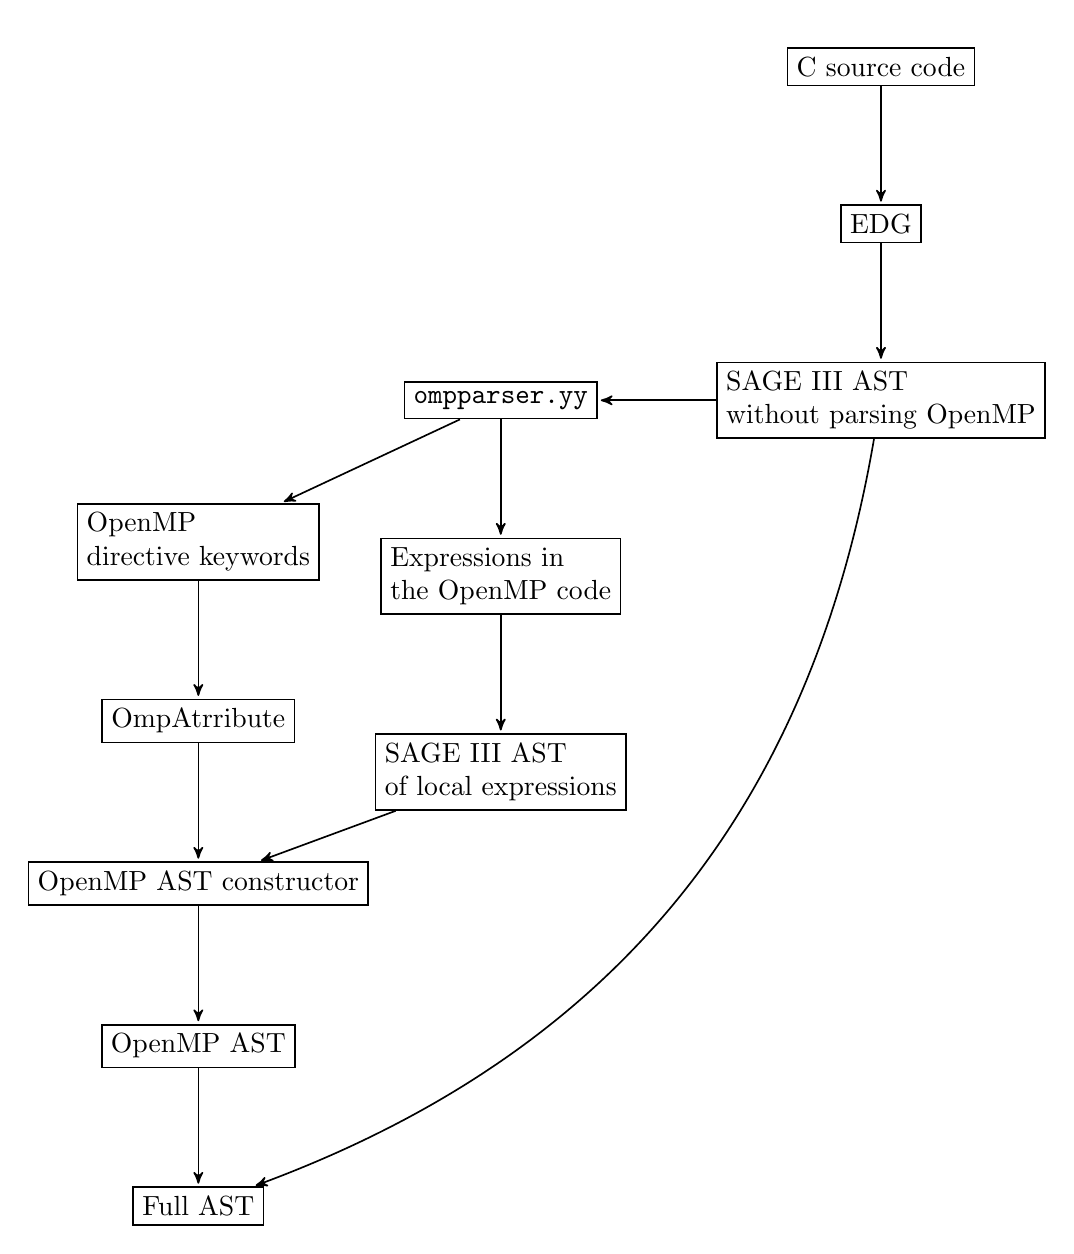
\begin{tikzpicture}[->,>=stealth',shorten >=1pt,auto,node distance=1.5cm,
                    semithick, every text node part/.style={align=left}]
  \tikzstyle{every state}=[fill=none,draw=black,text=black]

    \node[label = {$ $}, draw] (src)                    {C source code};
    \node[label = {$ $}, draw]         (edg) [below = of src] {EDG};
    \node[label = {$ $}, draw]         (ast0) [below = of edg] {SAGE III AST \\ without parsing OpenMP};
    \node[label = {$ $}, draw]         (ompparser) [left = of ast0] {\tt{ompparser.yy}};
    \node[label = {$ $}, draw]         (ompcode) [below left = of ompparser] {OpenMP\\ directive keywords};
    \node[label = {$ $}, draw]         (expr) [below = of ompparser] {Expressions in\\ the OpenMP code};

    \node[label = {$ $}, draw]         (ompattr) [below = of ompcode] {OmpAtrribute};
    \node[label = {$ $}, draw]         (exprast) [below = of expr] {SAGE III AST\\ of local expressions};
    \node[label = {$ $}, draw]         (ompastconstruct) [below = of ompattr] {OpenMP AST constructor};
    \node[label = {$ $}, draw]         (ompast) [below = of ompastconstruct] {OpenMP AST};
    \node[label = {$ $}, draw]         (fullast) [below = of ompast] {Full AST};




  \path (src) edge              node {$ $} (edg)
        (edg) edge              node {$ $} (ast0)
        (ast0) edge              node {$ $} (ompparser)
            edge [bend left]             node {$ $} (fullast)
        (ompparser) edge             node {$ $} (ompcode)
            edge              node {$ $} (expr)
        (ompcode) edge       node {$ $} (ompattr)
        (expr) edge       node {$ $} (exprast)
        (ompattr) edge       node {$ $} (ompastconstruct)
        (exprast) edge       node {$ $} (ompastconstruct)
        (ompastconstruct) edge       node {$ $} (ompast)
        (ompast) edge       node {$ $} (fullast);

\end{tikzpicture}

\caption{Standalone Design of OpenMP Parser}
\label{fig:ompparser}
\end{figure}

\end{document}

